\section{Common Stages in Deep Learning Approaches for Gesture Generation}
\label{sec:commonstage}

As presented in \autoref{sec:Data}, gestures consist of sequences of 3D point coordinates. For each dataset, the number of bones per frame may vary.

Deep learning approaches to gesture generation are implemented using various techniques. However, this thesis generalizes the process into the following main stages, illustrated in \autoref{fig:CommonStage}:

\begin{figure}[H]
	\centering
	\includegraphics[width=\textwidth]{CommonStage}
	\caption{Common stages in gesture generation models.}
	\label{fig:CommonStage}
\end{figure}

\begin{enumerate}[label=\textbf{\arabic*.}]
	\item \textbf{Preprocessing}: In the preprocessing stage, data such as speech segments, gesture sequences, and text are read and digitized into vectors or matrices that represent raw data information. Depending on the specific learning method, the selected initial data features may vary.

	\item \textbf{Feature Processing}: In this stage, raw data such as speech and text are embedded into feature vectors. Different methods use different embedding models. The way gesture sequences are represented as feature vectors also varies across methods.

	\item \textbf{Feature Extraction}: This stage uses linear transformation layers or CNN layers to extract features from the data. Text and speech features, after being processed, may be further passed through feature extraction layers to generate representation vectors corresponding to the input modalities.

	\item \textbf{Feature Encoding}: In this stage, gesture, emotion, and speech vectors are encoded into a lower-dimensional latent space to facilitate learning the correlations among modalities in the feature fusion stage.

	\item \textbf{Feature Fusion}: In this stage, features from speech, text, gestures, and other information are combined, typically using concatenation, fully connected layers, or operations such as vector addition or subtraction in the latent space.

	\item \textbf{Feature Decoding}: In this stage, latent vectors are decoded or upsampled back to their original dimensionality.

	\item \textbf{Rendering}: Once the output vectors are restored to their original size, they are converted back into BVH files and rendered using software such as Blender or Unity to visualize character motion.
\end{enumerate}

\section{Diffusion-based Model}
\label{sec:diffusionbase}

\subsection{General Principle of Diffusion-based Methods}

\begin{figure}[H]
	\centering
	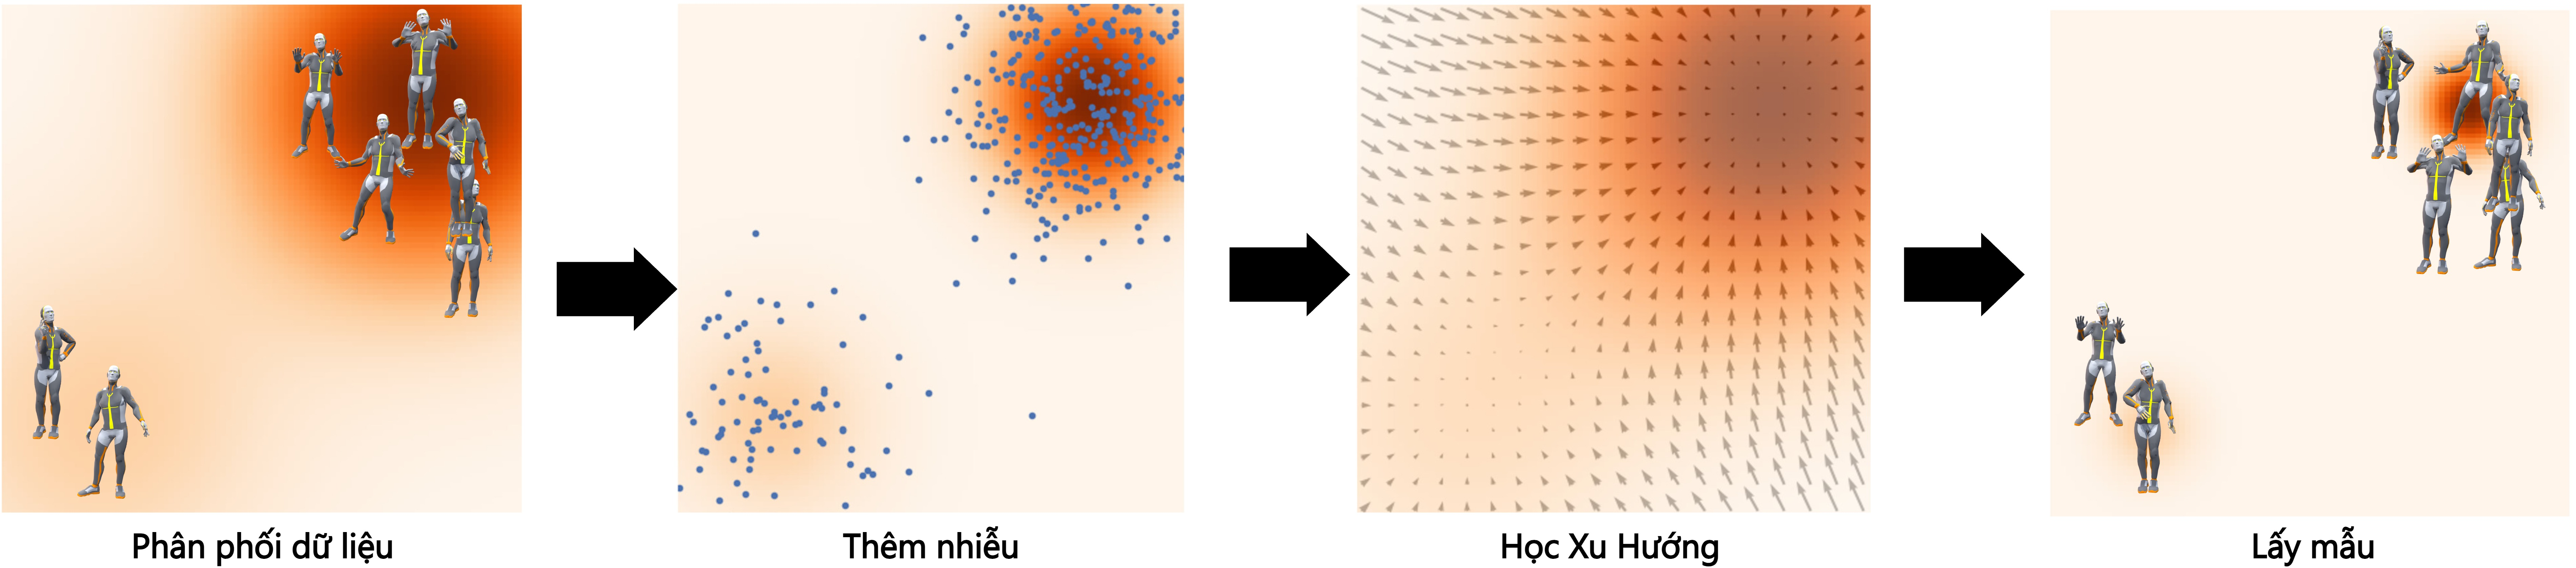
\includegraphics[width=\textwidth]{ScoreMatching}
	\caption{Illustration of the general principle of the Diffusion model.}
	\label{fig:ScoreMatching}
\end{figure}

Similar to the methods in the class of Implicit Generative Models (\autoref{sec:ImplicitGenerativeModels}), the core principle of Diffusion models is to learn a function $f_{\theta}$ that represents the drift process from a standard normal distribution $\mathcal{N}(0, \mathbf{I})$ to the data distribution $\bx_{0} \sim p(\bx)$. Sampling is performed step by step from this reverse process to generate new data, as illustrated in \autoref{fig:ScoreMatching}.

This process is executed over $T$ steps, with noise added at each step gradually reduced so that the model can navigate toward high-density regions of the data distribution.

\subsection{Typical Methods}
\label{subsec:TypicalMethod}


\subsubsection{Typical Methods}

\begin{itemize}
	\item \textit{MotionDiffuse} \cite{zhang2022motiondiffuse} employs a conditional Diffusion model, with conditions based solely on text, excluding audio. Additionally, the model predicts noise rather than directly predicting the original gesture sequence. MotionDiffuse utilizes Self-Attention and Cross-Attention layers to model the correlation between textual features and gesture features during \textit{Stage 5. Feature Fusion} (\autoref{fig:CommonStage}).
	
	\item \textit{Flame} \cite{kim2023flame} applies a Diffusion model with a Transformer-based architecture. In \textit{Stage 2. Feature Processing} (\autoref{fig:CommonStage}), it uses the pre-trained RoBERTa model to embed the text into textual feature vectors, which serve as the conditioning input. During \textit{Stage 5. Feature Fusion} (\autoref{fig:CommonStage}), the text is used as the $\texttt{CLS}$ token prepended to the gesture sequence before passing through the Transformer Decoder. Similar to other methods, the model predicts the added noise rather than the original gesture sequence.
	
	\item \textit{DiffWave} \cite{kong2020diffwave} is a noise-predicting Diffusion model in which the time steps pass through multiple Fully Connected layers and a Swish activation function before feature fusion. It uses a dilated convolutional architecture inherited from WaveNet. DiffWave enables better representation of speech, improving the effectiveness of conditioning for the Diffusion model.
	
	\item \textit{Listen, Denoise, Action} \cite{alexanderson2022listen} builds upon DiffWave \cite{kong2020diffwave}, replacing the dilated convolution layers with a Transformer, and integrating Conformer modules to enhance model performance.
	
	\item \textit{DiffSHEG} \cite{chen2024diffsheg} employs a Diffusion model; in \textit{Stage 2. Feature Processing}, it uses HuBERT to encode the audio signal. The model treats facial expressions as a signal for gesture generation and achieves real-time fusion of both facial expressions and gestures.
	
	\item \textit{GestureDiffuCLIP} \cite{ao2023gesturediffuclip} uses a Diffusion model conditioned on text, leveraging Contrastive Learning with CLIP to integrate text features and control gesture styles. Similar to other prompt-based approaches such as StableDiffusion or Midjourney, it treats text as prompts to learn gestures from descriptive sentences.
	
	\item \textit{Freetalker} \cite{yang2024freetalker} trains a Diffusion model on multiple datasets to generate speaker-specific gestures conditioned on speech and text. Unlike Transformer-based methods, Freetalker employs an Attention-based Network to model the correlation between textual, auditory, and gesture features during \textit{Stage 5. Feature Fusion} (\autoref{fig:CommonStage}).
\end{itemize}

\subsubsection{Inherited Method in This Thesis}

\begin{itemize}
	\item \textit{MDM} \cite{tevet2022human} applies conditional Diffusion to gesture generation, using CLIP (Contrastive Language–Image Pre-training) embeddings of descriptive text as conditions. MDM adopts a Transformer-based architecture to reconstruct original gesture data. Like other text-based Diffusion approaches, in \textit{Stage 3. Feature Extraction} (\autoref{fig:CommonStage}), the input text is randomly masked to hide certain segments, enabling the model to learn the importance of each part for various gestures. 
	
	In \textit{Stage 5. Feature Fusion} (\autoref{fig:CommonStage}), the text is prepended as a $\texttt{CLS}$ token to the gesture sequence before passing through the Transformer Encoder, where self-attention models the relationship between the text and each gesture frame. MDM predicts the original gesture data rather than noise.
	
	\item \textbf{DiffuseStyleGesture} \cite{yang2023diffusestylegesture} extends \textit{MDM} \cite{tevet2022human} by incorporating audio, initial gestures, and style as conditioning inputs. In \textit{Stage 1. Preprocessing} (\autoref{fig:CommonStage}), the model processes coordinate vectors to obtain feature vectors of dimension $D=1141$ per frame. In \textit{Stage 2. Feature Processing} (\autoref{fig:CommonStage}), DiffuseStyleGesture uses WavLM for audio embedding. In \textit{Stage 5. Feature Fusion} (\autoref{fig:CommonStage}), it improves upon MDM by applying Cross-Local Attention prior to the Transformer Encoder.
\end{itemize}

\subsection{Suitability of Diffusion Models for Gesture Generation}
\label{subsec:reason}

Given that gesture data consist of joint coordinates and rotational angles, they require high detail to ensure realistic character motion. However, data in extreme parameter cases are sparse. Thanks to their ability to capture fine-grained details and generalize to rare cases, Diffusion models are well-suited to address these challenges, as discussed in \autoref{sec:difficult}. A comparative evaluation of Diffusion models and other approaches is shown in \autoref{table:CompareMethod}.

This thesis selects Diffusion as the core model for the gesture generation task. Specifically, it adopts the \textbf{DiffuseStyleGesture} \cite{yang2023diffusestylegesture} model and integrates text as a semantic feature during \textit{Stage 5. Feature Fusion} (\autoref{fig:CommonStage}) in the gesture generation pipeline to propose the novel model \textbf{OHGesture}.
